The Volume/Balance module (\verb=Vol_Bal=) acts as the hub for processing incoming digital audio signals, forwarded from WM8731 via the \verb=Snd_Driver= module. As such, \verb=Vol_Bal= also keeps internal registers that holds current volume and balance levels as signed 4-bit values (legal values range from -5 to 5 where 0 represents no adjustment). These registers update via the one-hot coded input signal \verb=kb_input= applied by the \verb=Keyboard= module. Consequently, the values they hold are not only used as signals (\verb=i_volume_lvl=, \verb=i_balance_lvl=) for the internal submodules that process the \verb=LADC= and \verb=RADC= inputs, but also as module outputs connected to the \verb=VGA_Driver= so that they can be rendered on the screen.

\begin{figure}[h]
  \centering
  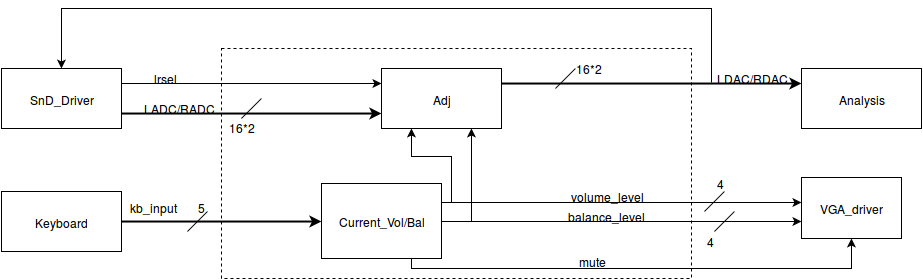
\includegraphics[width=16cm]{volbal}
  \caption{An overview of the Vol\_Bal module's internal workings.}
  \label{fig:vol_bal}
\end{figure}

The main function of the Volume/Balance module is to make requested adjustments to incoming values \verb=LADC= and \verb=RADC=, which represent measured amplitudes of the sound signal at distinct times. They will first be adjusted for volume by a function $A_{new} = A_{old} * \sqrt{2}^n$, where $A$ is the amplitude and $n$ is the signed value in the volume level register. The new values are forwarded for balance adjustment jointly with a \verb=ready= signal to inform that the \verb=adj_LADC= (or \verb=RADC=) should be read. Same processing is applied in the \verb=Bal_Adj= submodule to produce the \verb=LDAC= and \verb=RDAC= outputs conveyed to \verb=Snd_Driver= and \verb=Analysis=. Both adjustment submodules also use the input \verb=lrsel= as a control signal.

Ultimately, the user have the ability to digitally adjust the volume by -15/+15 dB and additionally balance it by decreasing volume by up to another 15 dB on a single left/right audio channel. There is also a mute function which is conveyed by \verb=kb_input=. When active, the register used as a ``mute enable'' essentially blanks any $A_{new}$ values on the \verb=LDAC/RDAC= outputs.


